% !TeX root = ../main.tex
% Add the above to each chapter to make compiling the PDF easier in some editors.

\chapter{Effective Resistance}\label{cha:effective_resistance}

\begin{defn}[Effective resistance] The \emph{effective resistance}\index{effective resistance}, \begin{align}
    \Reff(a,b) \defeq \min_{\substack{\vf \in \R^{|\sE|} \\ \mB\vf = \vOne_b - \vOne_a}} \mathcal{E}(\vf),
\end{align} is the minimum electrical energy required to route one unit of flow from $a$ to $b$.
\end{defn}
\begin{rmk}
Per definition of electrical energy, routing $F$ units of flow from $a$ to $b$ costs $F^2 \Reff(a,b)$.
\end{rmk}

\begin{lem}
$\Reff(a,b) = \norm{\mL^{\nicefrac{+}{2}}(\vOne_b - \vOne_a)}_2^2$.
\end{lem}
\begin{proof} As the electrical flow $\ef$ is energy-minimizing, we have that $\Reff(a,b) = \trans{\ef}\mR\ef$. Recall that by Ohm's law this flow corresponds to voltages $\ex$ solving $\mL\ex = \vOne_b - \vOne_a$, that is, $\ex = \pinv{\mL}(\vOne_b - \vOne_a)$. We obtain, \begin{align*}
    \Reff(a,b) = \trans{\ef}\mR\ef = \trans{\ex}\mL\ex &= \trans{(\vOne_b - \vOne_a)}\pinv{\mL}\mL\pinv{\mL}(\vOne_b - \vOne_a) \\
    &= \trans{(\vOne_b - \vOne_a)}\pinv{\mL}(\vOne_b - \vOne_a) \margintag{using that $\vOne_b - \vOne_a \perp \vOne$} \\
    &= \norm{\mL^{\nicefrac{+}{2}}(\vOne_b - \vOne_a)}_2^2. \qedhere
\end{align*}
\end{proof}

\begin{lem}
If $G$ is a $\phi$-expander, then \begin{align}
    \Reff(a,b) \leq 2\phi^{-2}\parentheses*{\frac{1}{\vd(b)} + \frac{1}{\vd(a)}}.
\end{align}
\end{lem}
\begin{proof}
By Cheeger's inequality, \begin{align*}
    \phi \leq \phi(G) \leq \sqrt{2 \lambda_2(\mN)} \implies \frac{\phi^2}{2} \leq \lambda_2(\mN).
\end{align*} By Courant-Fischer, we have that for any $\vy \perp \ker{\mN}$, \begin{align*}
    \frac{\phi^2}{2} \leq \lambda_2(\mN) \leq \frac{\trans{\vy}\mN\vy}{\trans{\vy}\vy} \implies \frac{\phi^2}{2}\trans{\vy}\vy \leq \trans{\vy}\mN\vy.
\end{align*} Equivalently, \begin{align*}
    \frac{\phi^2}{2}\mPi_\mN \preceq \mN, \margintag{using that $\mPi_\mN \vv = \vv$ for $\vv \perp \ker{\mN}$, and $\mPi_\mN \vv = 0$ if $\vv \in \ker\mN$}
\end{align*} where $\mPi_\mN$ is the projection orthogonal to the kernel of $\mN$. From this we conclude that \begin{align*}
    2\phi^{-2}\mPi_\mN = 2\phi^{-2}\pinv{\mPi_\mN} \succeq \pinv{\mN}, \margintag{using $\pinv{\mPi_\mN} = \mPi_\mN$}
\end{align*} as $\mA \succeq \mB$ implies $\pinv{\mA} \preceq \pinv{\mB}$ when $\ker\mA = \ker\mB$. By \cref{eq:pinv_calculation}, \begin{align}
    \pinv{\mN} = \pinv{(\mD^{-\nicefrac{1}{2}}\mL\mD^{-\nicefrac{1}{2}})} = \mPi_\mN\mD^{\nicefrac{1}{2}}\pinv{\mL}\mD^{\nicefrac{1}{2}}\mPi_\mN
\end{align} Therefore, for any $\vy \perp \ker\mN$, \begin{align*}
    2\phi^{-2}\trans{\vy}\vy \geq \trans{\vy}\pinv{\mN}\vy = \trans{\vy}\mD^{\nicefrac{1}{2}}\pinv{\mL}\mD^{\nicefrac{1}{2}}\vy.
\end{align*} Substituting $\vz \defeq \mD^{-\nicefrac{1}{2}}\vy$, we obtain, \begin{align*}
    2\phi^{-2}\trans{\vz}\inv{\mD}\vz \geq \trans{\vz}\pinv{\mL}\vz.
\end{align*} Finally, observe that for $\vz \defeq \vOne_b - \vOne_a$, we have that $\vy = \mD^{\nicefrac{1}{2}}(\vOne_b - \vOne_a) \perp \ker\mN$ as $\vOne_b - \vOne_a \perp \ker\mL$ and therefore,\footnote{We have for the kernel of the normalized Laplacian matrix, $\mN = \mD^{-\nicefrac{1}{2}}\mL\mD^{-\nicefrac{1}{2}}$, that $\ker\mN = \mD^{\nicefrac{1}{2}}\ker\mL = \vspan\{\mD^{\nicefrac{1}{2}}\vOne\}$.} \begin{align*}
    \Reff(a,b) = \trans{\vz}\pinv{\mL}\vz \leq 2\phi^{-2}\trans{\vz}\inv{\mD}\vz = 2\phi^{-2}\parentheses*{\frac{1}{\vd(b)} + \frac{1}{\vd(a)}}. &\qedhere
\end{align*}
\end{proof}

\begin{lem}
$\E{C_{a,b}} = \norm{\vd}_1 \Reff(a,b)$.
\end{lem}
\begin{proof} Recall that $\E{C_{a,b}} = \trans{(\vOne_a - \vOne_b)}\ex$ for a solution $\ex$ to $\mL\ex = \norm{\vd}_1 (\vOne_a - \vOne_b)$, that is, $\ex = \norm{\vd}_1\pinv{\mL}(\vOne_a - \vOne_b)$. Now, observe that, \begin{align*}
    \Reff(b,a) = \trans{(\vOne_a - \vOne_b)}\pinv{\mL}(\vOne_a - \vOne_b) = \frac{1}{\norm{\vd}_1}\trans{(\vOne_a - \vOne_b)}\ex.
\end{align*} Thus, $\E{C_{a,b}} = \norm{\vd}_1 \Reff(b,a)$. Using symmetry of the commute time, $\E{C_{a,b}} = \E{C_{b,a}} = \norm{\vd}_1 \Reff(a,b)$.
\end{proof}

\begin{cor}\label{cor:effective_resistance_symmetric}
Effective resistance is symmetric.
\end{cor}

Let us consider a few examples.

\begin{marginfigure}
TBD
% \centering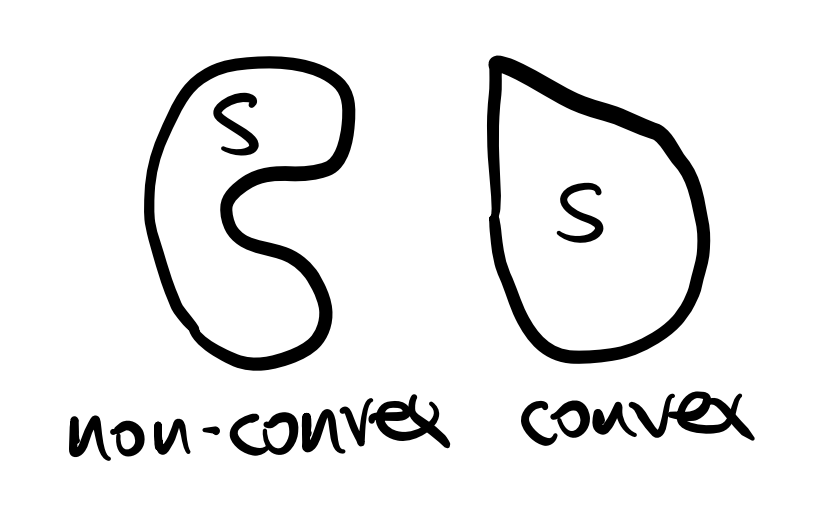
\includegraphics[width=4cm]{notes/figures/convex_set.png}
\caption{Sequential resistors.}\label{fig:sequential_resistors}
\end{marginfigure}
\begin{lem}
For the graph of \cref{fig:sequential_resistors}, $\Reff(1,k+1) = \sum_{i=1}^k \vr(i)$.
\end{lem}
\begin{proof}[Proof sketch] For the flow to be $1$, by Ohm's law, the voltage difference across edge $i$ must be $\vr(i)$.
\end{proof}

\begin{marginfigure}
TBD
% \centering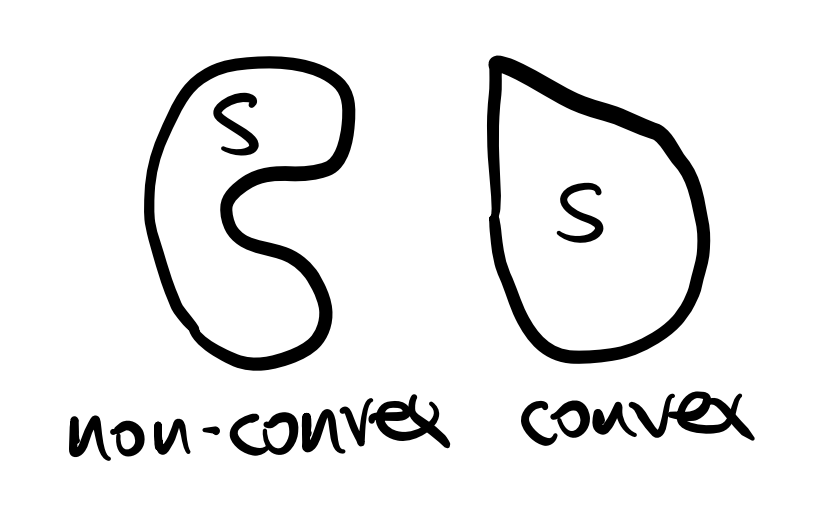
\includegraphics[width=4cm]{notes/figures/convex_set.png}
\caption{Parallel resistors.}\label{fig:parallel_resistors}
\end{marginfigure}
\begin{lem}
For the graph of \cref{fig:parallel_resistors}, $\Reff(1,2) = \frac{1}{\sum_{i=1}^k \nicefrac{1}{\vr(i)}}$.
\end{lem}
\begin{proof}[Proof sketch] For the flow to be $1$, by Ohm's law, we must have, \begin{align*}
    1 = \sum_{i=1}^k \frac{\ex(\{1,2\})}{\vr(i)},
\end{align*} where $\ex(\{1,2\})$ is the voltage difference between vertices $1$ and $2$. Note that $\Reff(1,2) = \ex(\{1,2\})$.
\end{proof}

\section{Effective Resistance as a Metric}

Before showing that effective resistance is a metric on the set of vertices, we consider the following lemma. We will write, \begin{align}
    \ex_{a,b} \defeq \pinv{\mL}(\vOne_b - \vOne_a),
\end{align} for the electrical voltages required to route one unit of current from $a$ to $b$.

\begin{lem}\label{lem:voltages_are_weighted_average}
If $\ex_{a,b}$ is a solution to $\mL\ex_{a,b} = \vOne_b - \vOne_a$, then we have for all $c \in \sV$ that $\ex_{a,b}(b) \geq \ex_{a,b}(c) \geq \ex_{a,b}(a)$.
\end{lem}
\begin{proof}[Proof sketch] Consider any $c \in \sV \setminus \{a,b\}$. Then, $(\mL\ex_{a,b})(c) = 0$. Thus, \begin{align*}
    \parentheses*{\sum_{v \sim c} \vw(\{v,c\})} \ex_{a,b}(c) - \parentheses*{\sum_{v \sim c} \vw(\{v,c\}) \ex_{a,b}(v)} = 0.
\end{align*} So, we have, \begin{align*}
    \ex_{a,b}(c) = \frac{\sum_{v \sim c} \vw(\{v,c\}) \ex_{a,b}(v)}{\sum_{v \sim c} \vw(\{v,c\})}.
\end{align*} In words, the electrical voltage of $c$ is a weighted average of the voltages of its neighbors. It follows that the voltages of $a$ and $b$ take the largest absolute values.
\end{proof}

\begin{defn}[Metric] A \emph{metric}\index{metric} on a set $\sS$ is a function $d : \sS \times \sS \to \R$ such that for any $a, b, c \in \sS$, \begin{enumerate}
    \item $d(a,b) = 0 \iff a = b$;
    \item $d(a,b) \geq 0$;
    \item $d(a,b) = d(b,a)$; and
    \item $d(a,b) \leq d(a,c) + d(c,b)$.
\end{enumerate}
\end{defn}
\begin{lem}
Effective resistance is a metric on $\sV$.
\end{lem}
\begin{proof} It is easy to check that properties (1) and (2) are satisfied. We have that property (3) is satisfied by \cref{cor:effective_resistance_symmetric}.

Let us therefore consider property (4), the triangle inequality. We have, \begin{align*}
    \ex_{a,b} = \pinv{\mL}(\vOne_b - \vOne_a) = \pinv{\mL}(\vOne_c - \vOne_a + \vOne_b - \vOne_c) = \ex_{a,c} + \ex_{c,b},
\end{align*} This we can use to rephrase the effective resistance, \begin{align*}
    \Reff(a,b) = \trans{(\vOne_b - \vOne_a)}\ex_{a,b} &= \trans{(\vOne_b - \vOne_a)}(\ex_{a,c} + \ex_{c,b}) \\
    &= \ex_{a,c}(b) - \ex_{a,c}(a) + \ex_{c,b}(b) - \ex_{c,b}(a) \\
    &\leq \ex_{a,c}(c) - \ex_{a,c}(a) + \ex_{c,b}(b) - \ex_{c,b}(c) \margintag{using \cref{lem:voltages_are_weighted_average}} \\
    &= \trans{(\vOne_c - \vOne_a)}\ex_{a,c} + \trans{(\vOne_b - \vOne_c)}\ex_{c,b} \\
    &= \Reff(a,c) + \Reff(c,b). \qedhere
\end{align*}
\end{proof}